\documentclass{article}
\usepackage{indentfirst}
\usepackage{blindtext}
\usepackage{graphicx}
\usepackage{wrapfig}
\graphicspath{ {./images/uart/} }

\title{Skills Assessment}
\author{Nathan Givens}
\date{November 8, 2019}

\setlength{\parindent}{4ex}

\begin{document}

  \maketitle

  \section{UART Bus Decoding}

  \subsection{Required Equipment}

  UART bus decoding is a method of capturing communications over a UART bus and
  decoding the information sent between devices. Equipment often decodes the
  information into hexadecimal, but the equipment we have available can display
  the information in binary and ASCII as well. The procedure described in this
  document should apply to any of the oscilloscopes available in the senior
  design labs but was prepared using a Keysight MS0-X 3014T so there may be
  some subtle differences between models.

  \begin{figure}[h]
    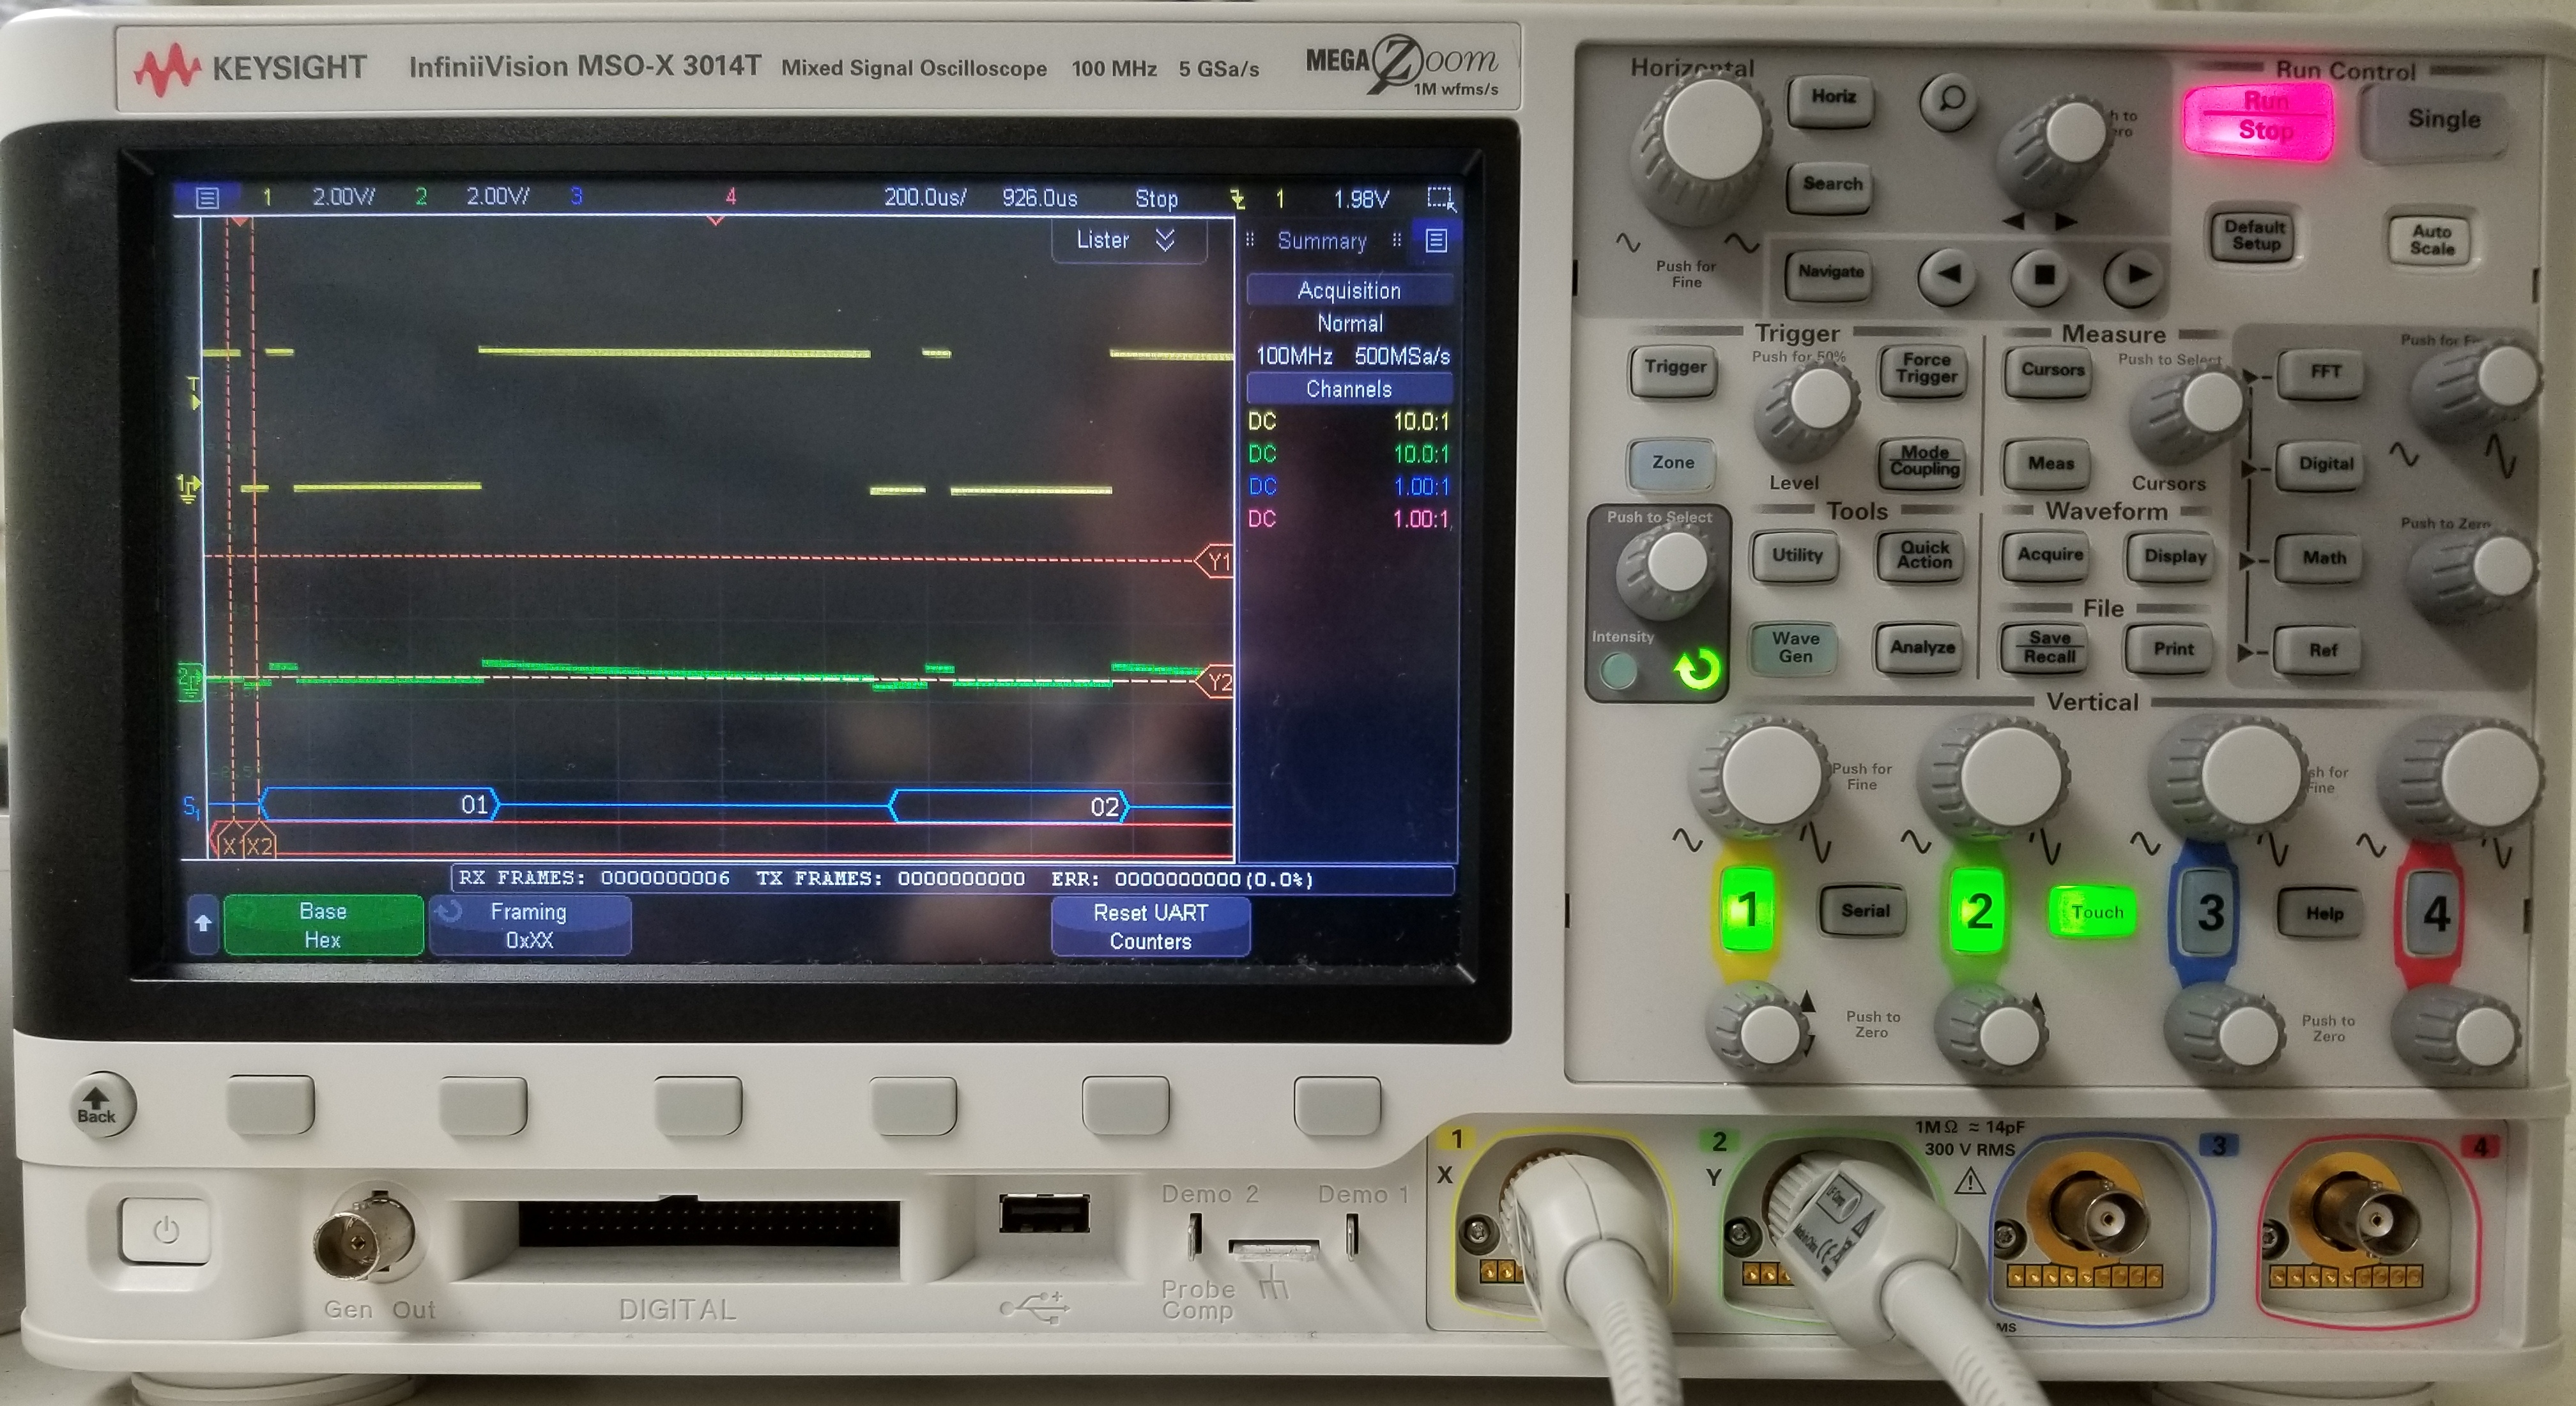
\includegraphics[width=\textwidth]{full_scope}
    \caption{An oscilloscope properly decoding data from a UART bus}
  \end{figure}

  \subsection{Making the Measurement}

  Firstly, the oscilloscope must be turned on and the proper number of probes
  must be connected. For UART, two cables are needed to test two way
  asynchronous communications. If only one signal needs to be decoded, then only
  one cable needs to be connected to the oscilloscope. However, having more
  cables connected to the oscilloscope won't hurt anything, it just clutter up
  your area.

  \begin{wrapfigure}{l}{44ex}
    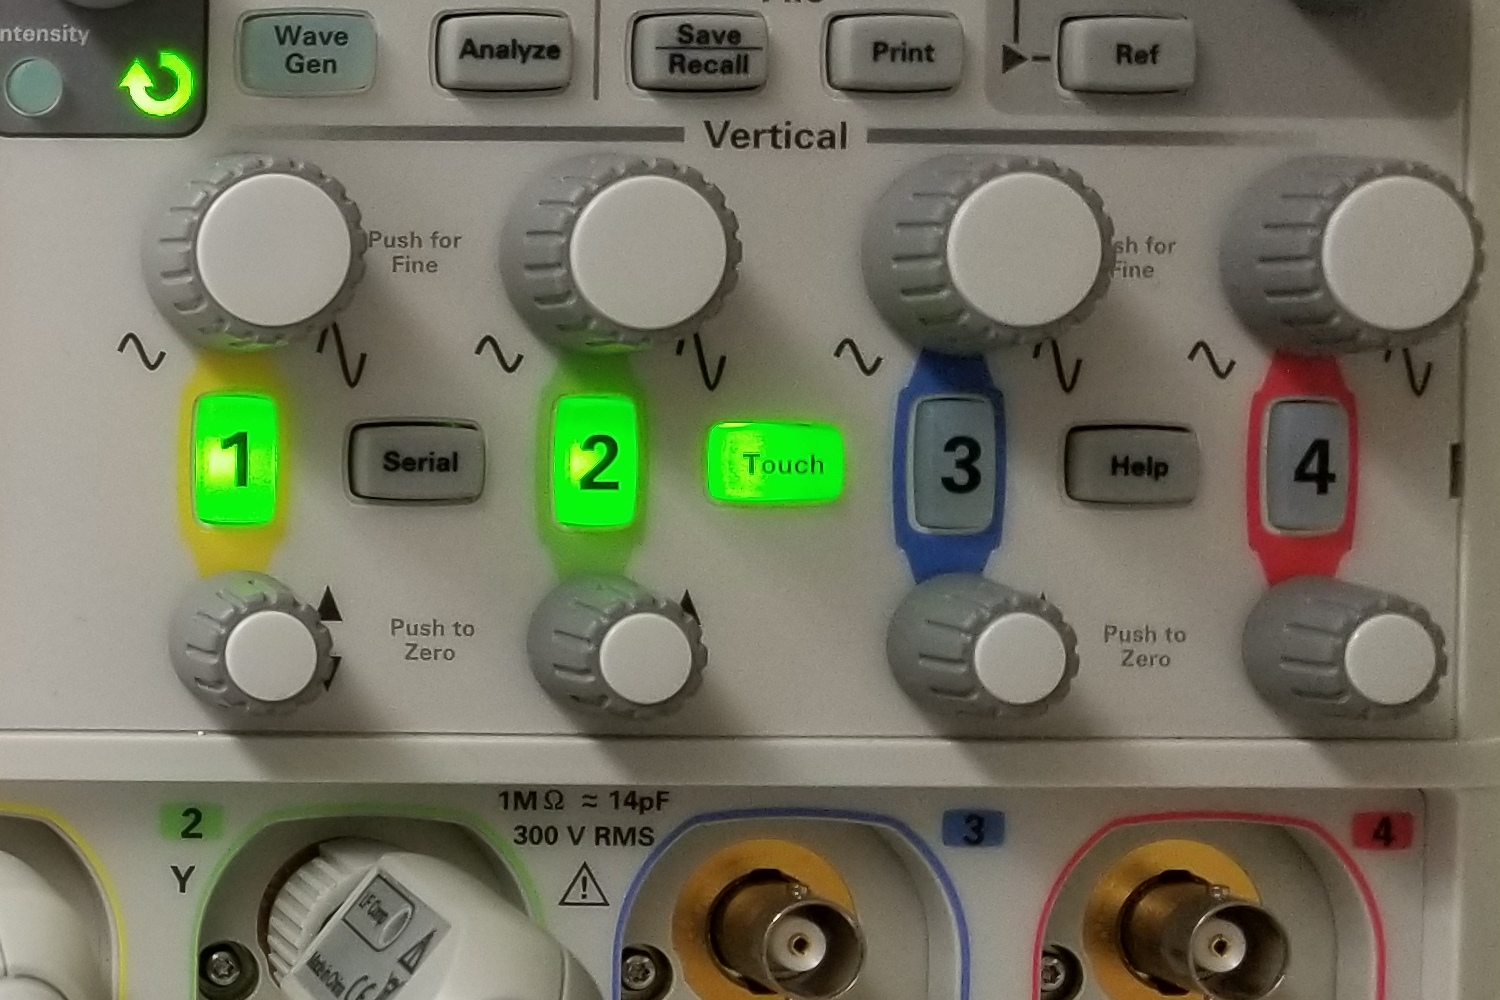
\includegraphics[width=44ex]{serial_button_scope}
    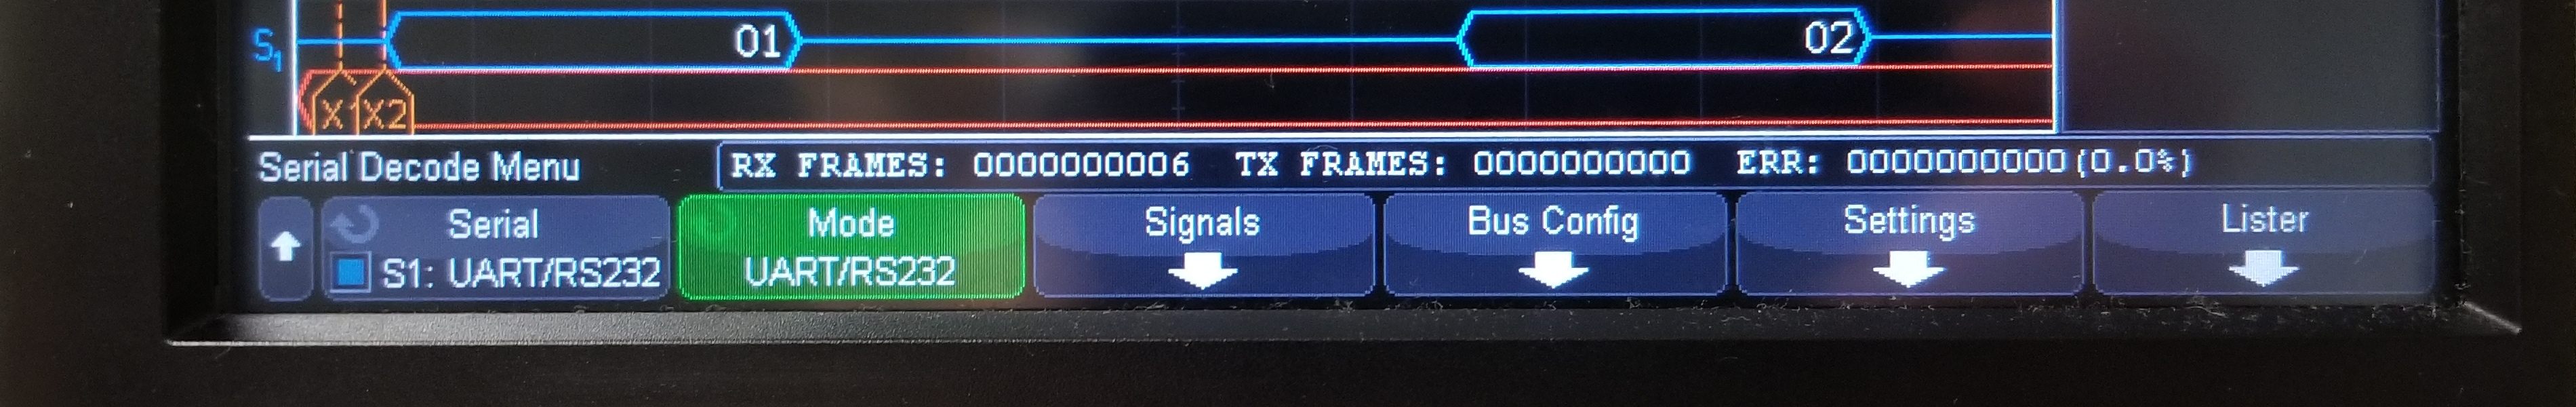
\includegraphics[width=44ex]{serial_decode_scope}
    \caption{Serial button located between buttons 1 and 2. Serial Decode Menu,
      shown with UART/RS232 selected.}
  \end{wrapfigure}

  The oscilloscopes have a Serial button located between buttons 1 and 2.
  Pressing this button opens the serial protocol decoding menu at the bottom of
  the display. The menu changes according to the selected protocol. This menu
  holds all of the settings associated with serial bus deocing. This
  document will discuss some of the various settings that are available, and
  walk through an example of configuring the scope to properly decode a UART bus
  communication.

  \begin{wrapfigure}{r}{25ex}
    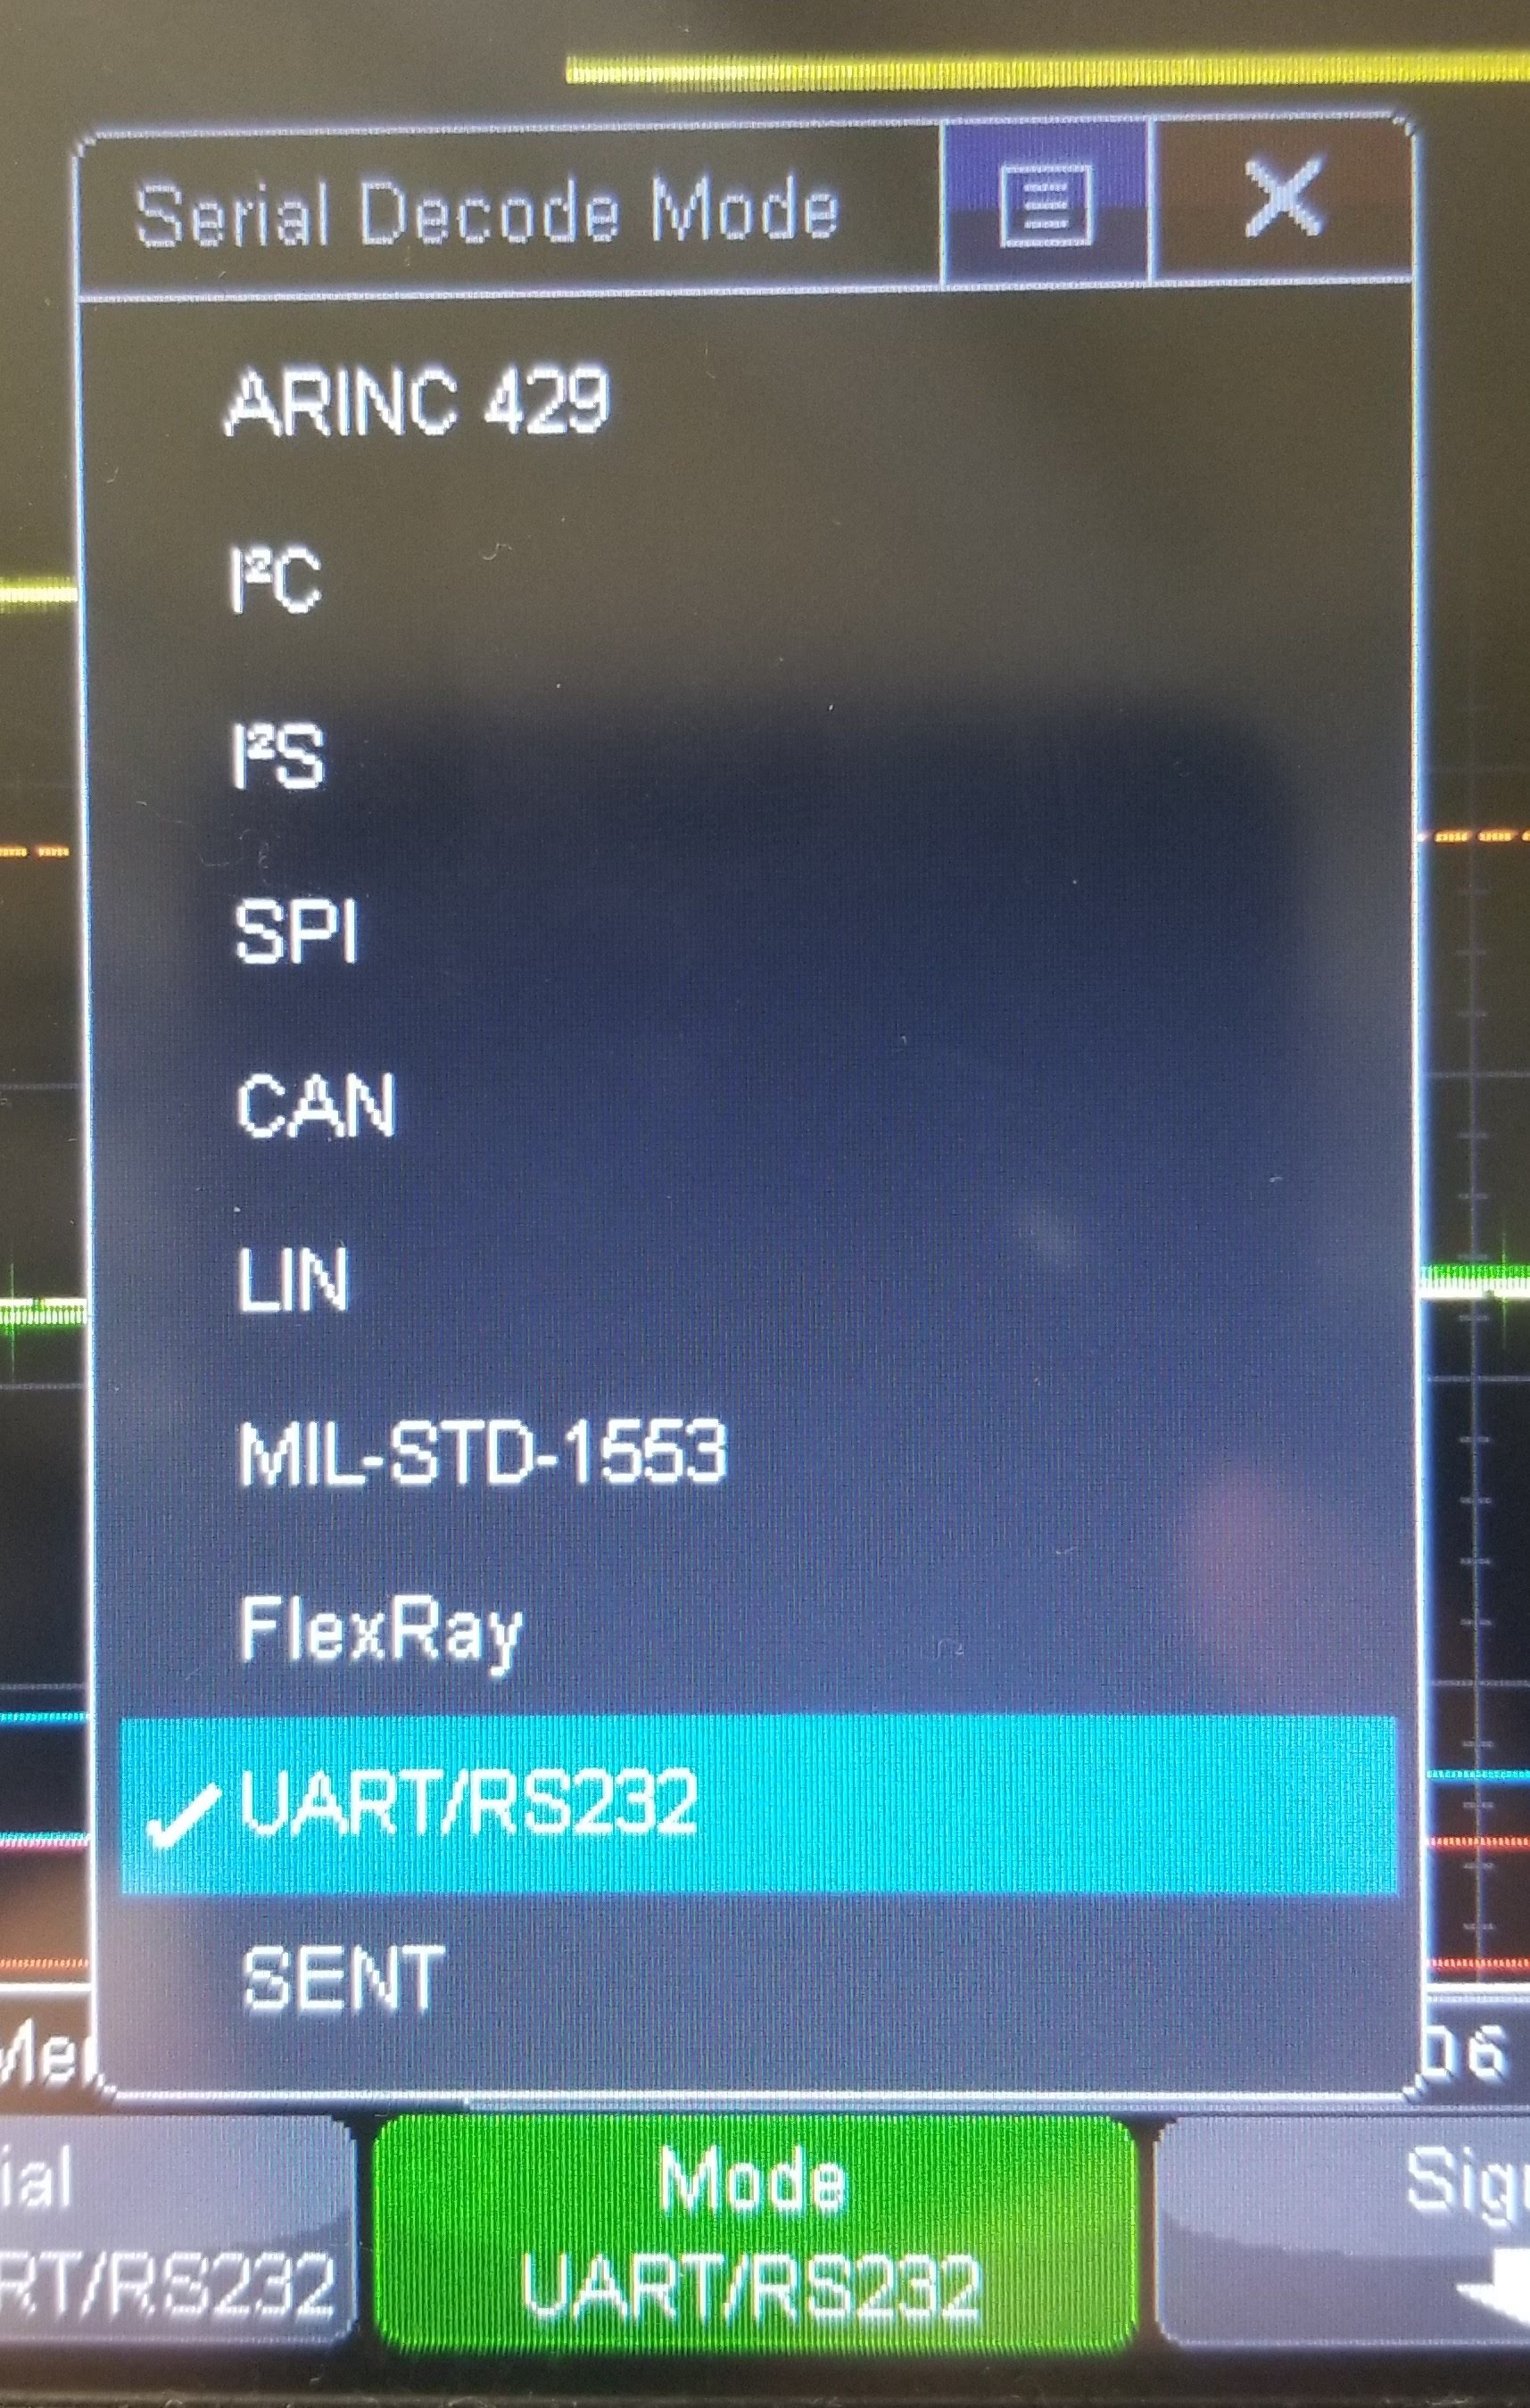
\includegraphics[width=25ex]{mode_menu}
    \caption{Mode selection menu on oscilloscope}
    \label{fig:uart_mode_menu}
  \end{wrapfigure}

  Inside the serial menu, the mode needs to be set to reflect the expected
  communication. Conveniently, the mode button allows this configuration to be
  made. Pressing the mode button reveals a list of communication protocols that
  the oscilloscope can decode. Because this section describes UART communication
  decoding, UART/RS232 is selected from the list. Other sections of this
  document discuss some of the other protocols listed here. After UART/RS232 is
  selected, all submenus update to display settings
  specific to decoding UART.\@

  % Signals submenu
  The signals submenu gives the ability to specify which input is associated
  with which signal. In the case of UART, the availbalbe signals are Rx and Tx.
  In the example, channel 1 is set to Rx and receives the signals that are
  leaving through the devices Tx connection. The channel could be connected to
  either Rx or Tx from the device, but sticking with convention should help to
  prevent confusion while debugging. The thresholds for signals can also be
  adjusted here in case different voltages are being used. The threshold shown
  in Figure~\ref{fig:uart_signals_menu} for Rx was set to just above the threshold
  for logic high in the device meant to receive the signals. The Tx signal was
  not set because, for this example, there was no Tx signal connected. Now that
  the oscilloscope knows which signal is connected to which channel, the bus
  settings can be configured so signals can be properly decoded.

  \begin{figure}[h]
    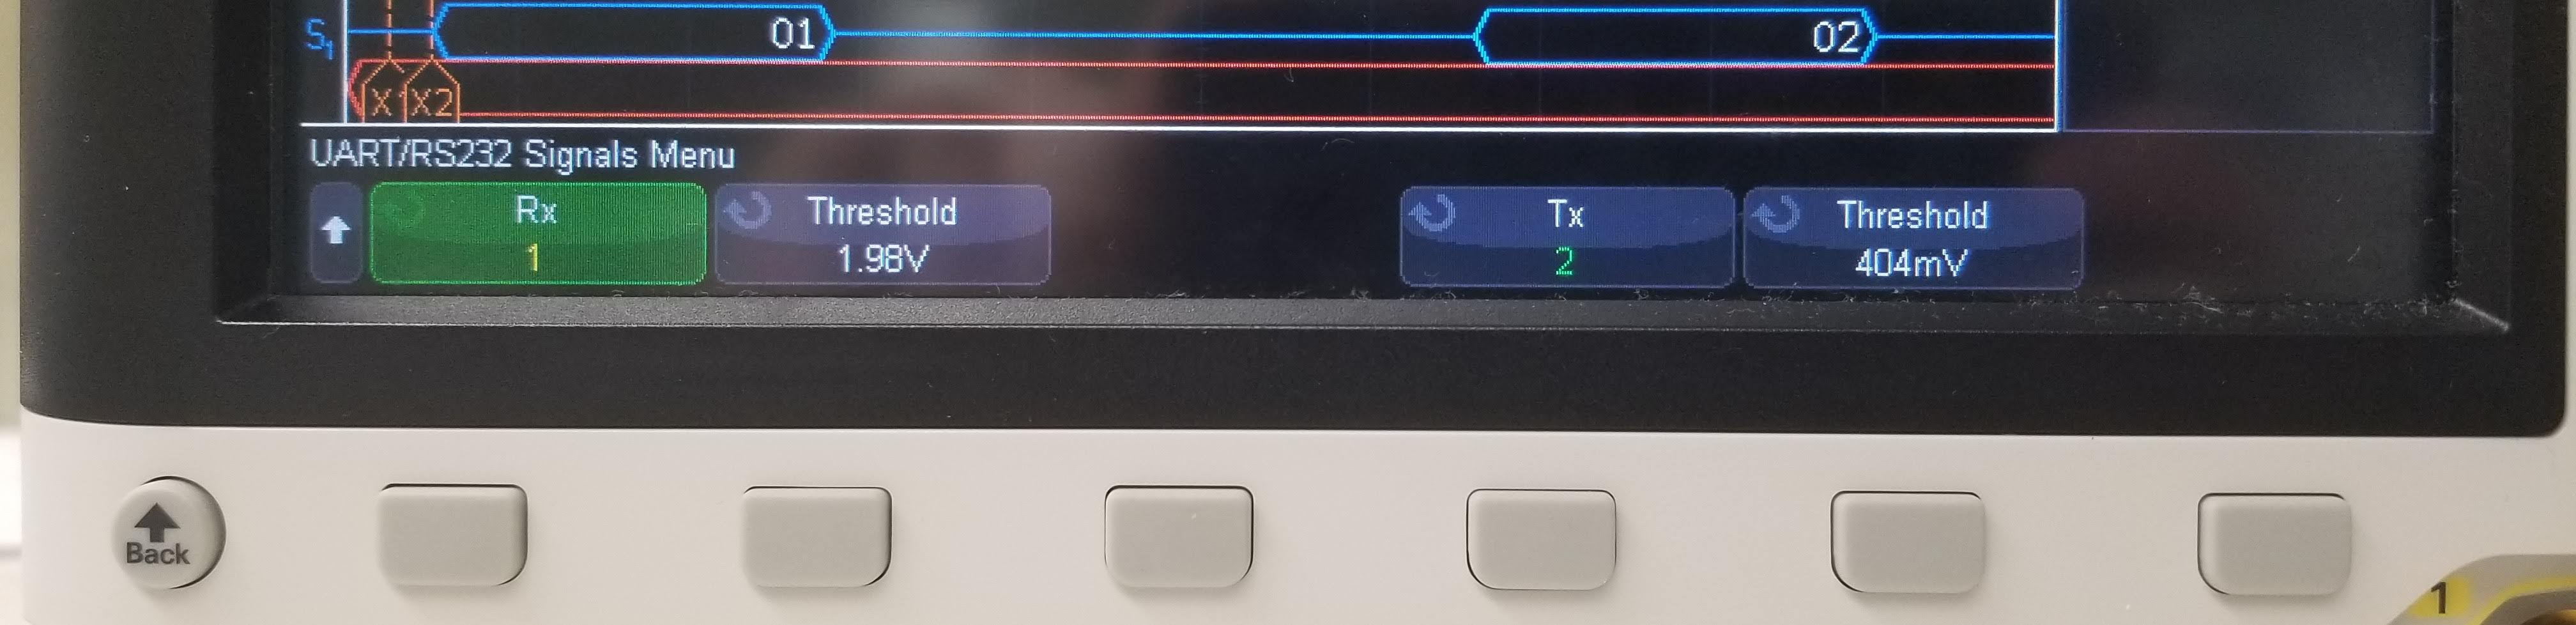
\includegraphics[width=\textwidth]{signals_menu}
    \caption{Signals submenu showing channel 1 as Rx with a threshold of 1.98V}
    \label{fig:uart_signals_menu}
  \end{figure}

  % Bus Configuration
  The configurations for UART communication are located in the Bus Config Menu.
  The number of bits, parity (if any), baud rate, idle polarity, and bit order
  can be adjusted here to match the expected transmission settings. The baud
  rate is adjusted from within a submenu where a value can be entered directly.
  This example uses eight bit transmissions without a parity bit. An idle line
  should remain at logic high, and the bits are transmitted Least Significant
  Bit first. This was also recorded at 19,200 baud.

  \begin{figure}[h]
    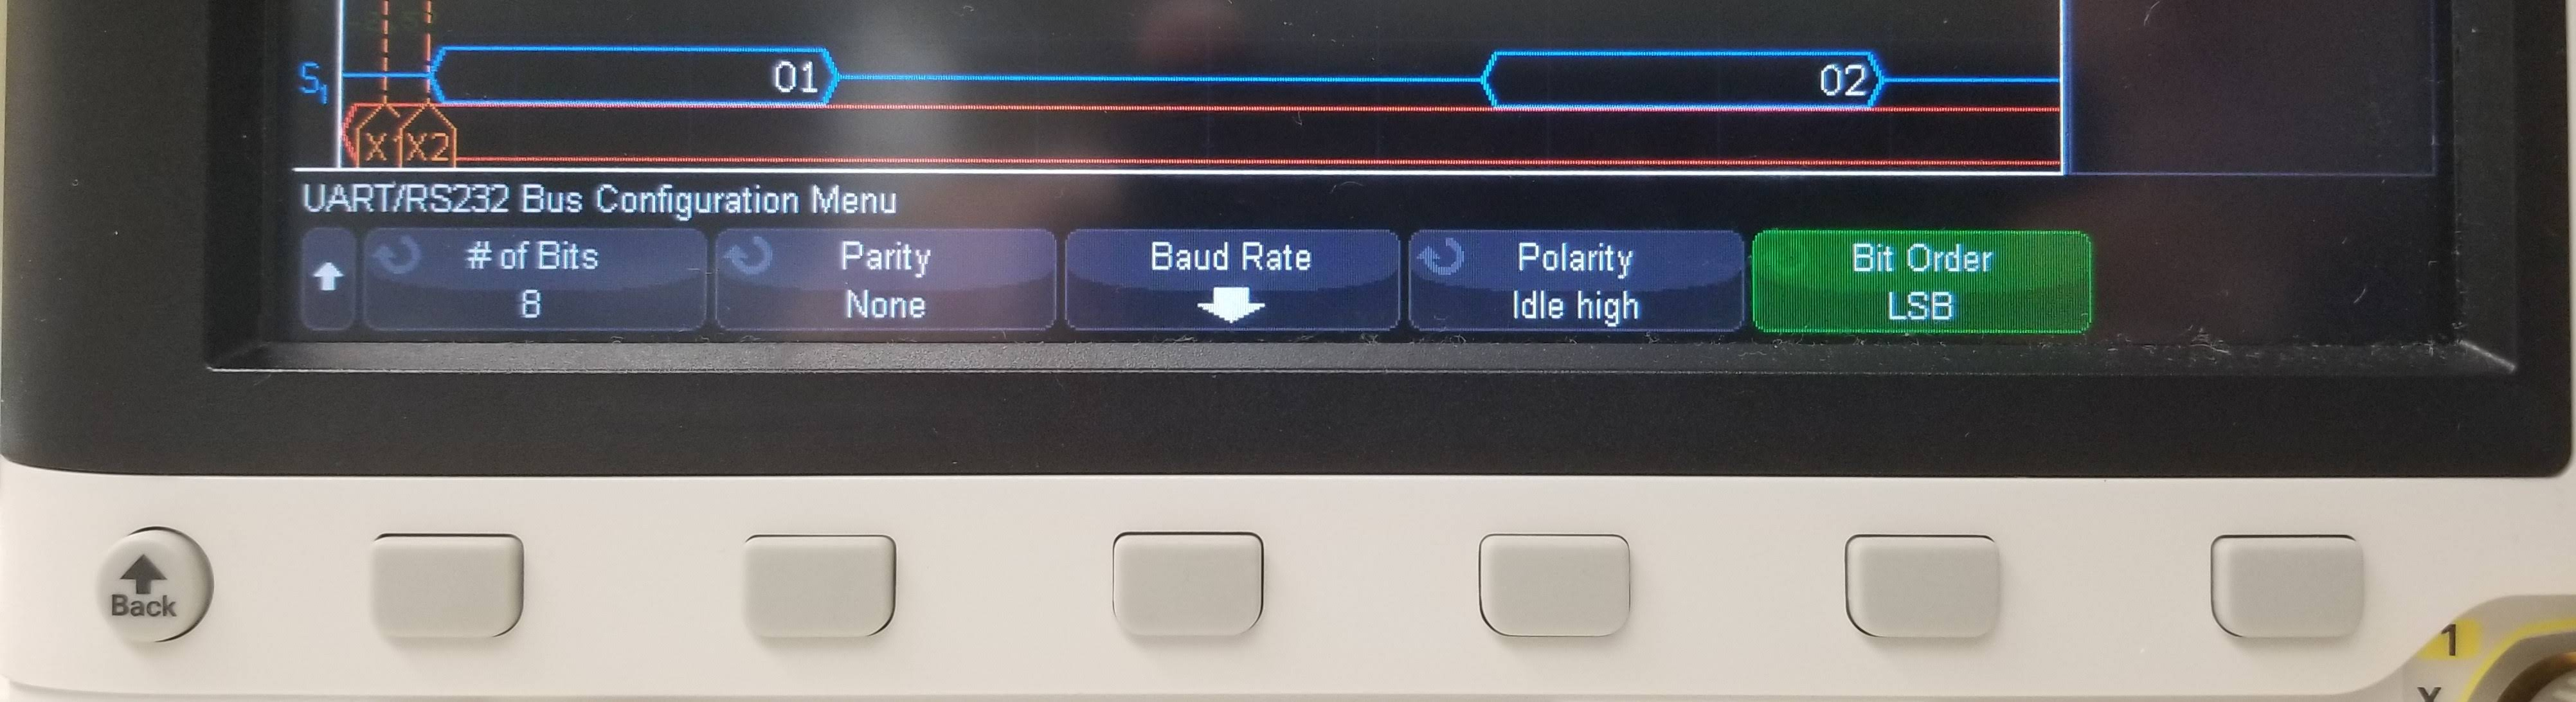
\includegraphics[width=\textwidth]{bus_config}
    \caption{UART/RS232 Bus Configuration Menu}
  \end{figure}

  \clearpage

  % Settings
  Inside the settings menu, the base number for displayed values can be
  selected. The example is currently set to hex, so all numbers displayed are
  hexadecimal. The framing size for displayed information can also be adjusted.
  Currently, the framing size is set to two, so the information is broken into
  two hexadecimal numbers per frame. This was chosen in the example because it
  matches the size of data frames that are sent. The oscilloscope will also keep
  a running total of frames it has received, and the last button in this submenu
  can reset that running total. This can be useful to ensure the proper number
  of data frames when trying to decode long message sequences.

  \begin{figure}[ht]
    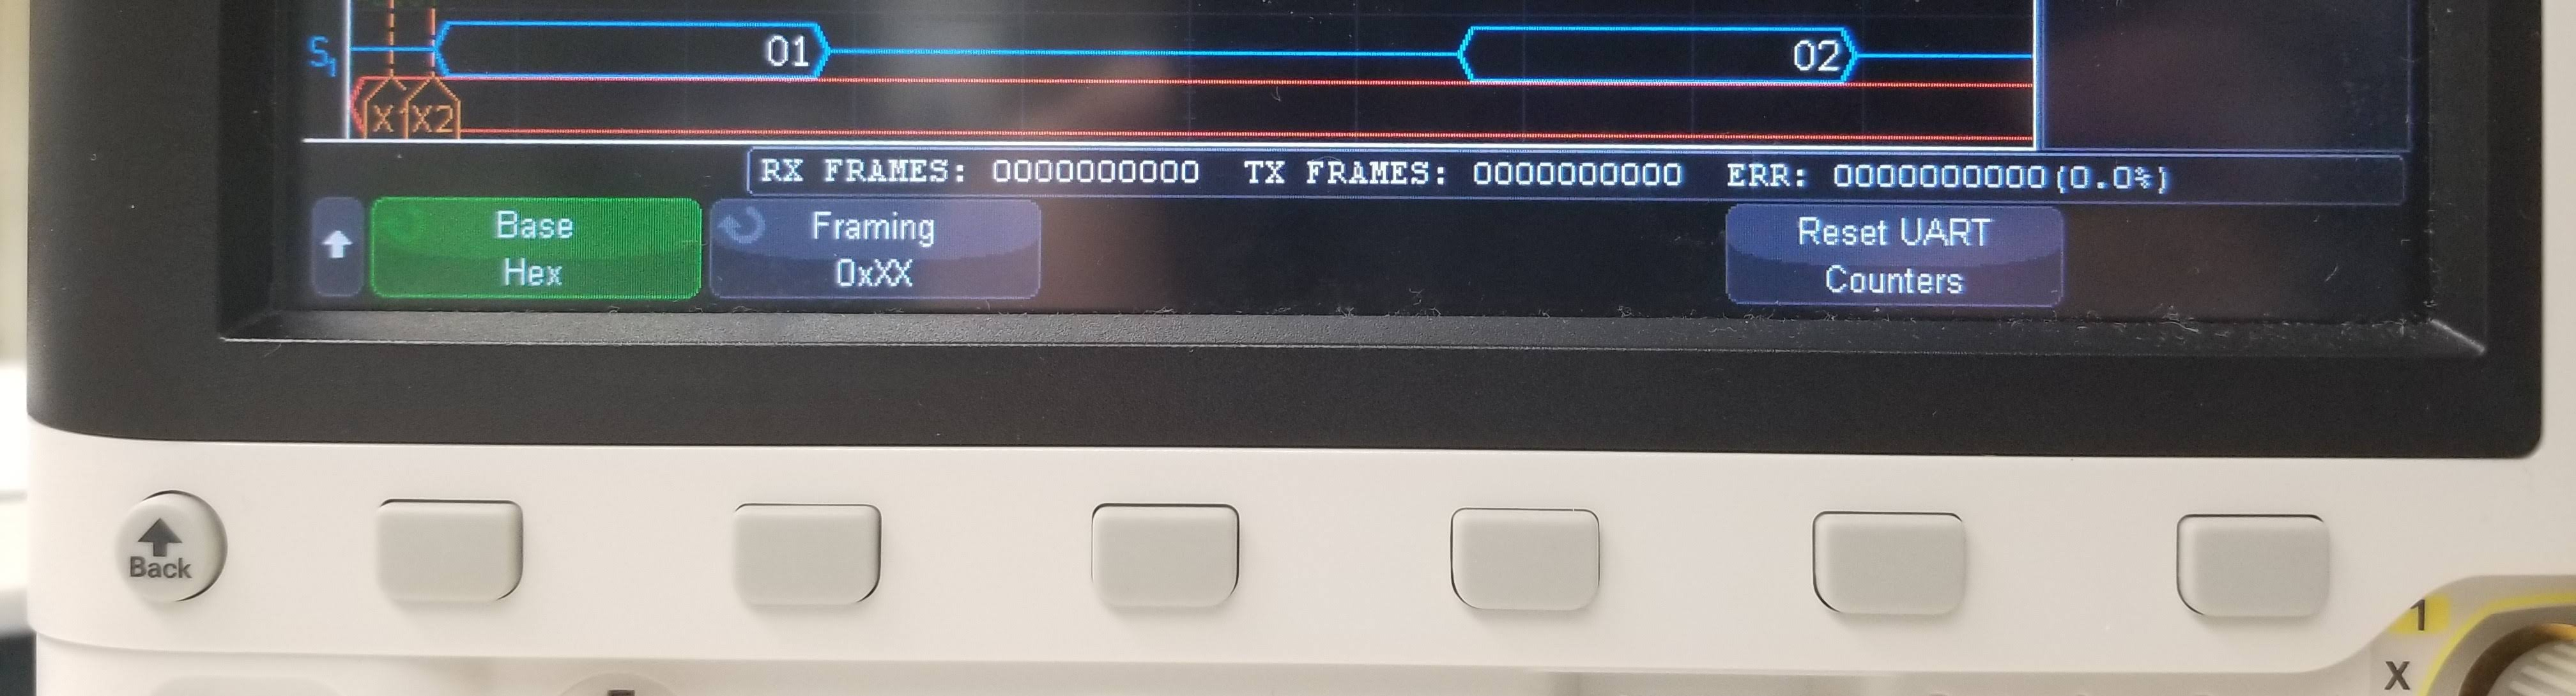
\includegraphics[width=\textwidth]{setting}
    \caption{Settings submenu for UART configuration}
  \end{figure}

  \subsection{Measurements}

  \begin{figure}[ht]
    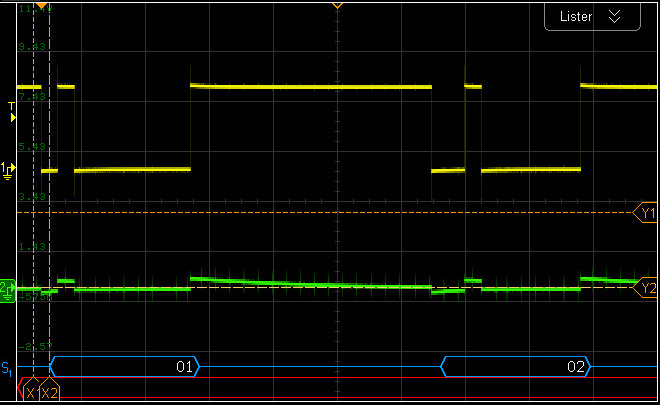
\includegraphics[width=\textwidth]{uart_bus}
    \caption{Decoded UART Signals}
    \label{fig:uart_bus}
  \end{figure}

  When the oscilloscope detects a data frame, it will decode the signals it
  receives and display those values at the bottom of the screen as shown in
  Figure~\ref{fig:uart_bus}. The blue signals represent the Rx signals that were
  decoded. If a Tx signal had been measured, its values would be displayed in
  the red signals at the bottom of the screen. Figure~\ref{fig:uart_bus} shows
  0x01 and 0x02 data frames were received, and those were in fact the expected
  signals.

  \section{SPI Bus Decoding}

  \subsection{Required Equipment}

  The oscilloscopes available in the labs can also be used to decode SPI Bus
  communications. The configuration process is similar to that used for UART decoding,
  so it will be covered in slightly less detail in this section.

\end{document}
